\documentclass[conference,compsoc]{IEEEtran}


\usepackage[pdftex]{graphicx}
\usepackage{amsmath}
\usepackage{xcolor}
\usepackage{tikz}
\usepackage{schemabloc}
\usepackage{multicol}
\usepackage{amssymb}
\usepackage{enumerate}
\usetikzlibrary{circuits}
\usetikzlibrary{calc}
\usetikzlibrary{shapes,shadows,arrows}

%------------------------------------> To create hyperlinks
\usepackage[colorlinks=true, linkcolor=black, citecolor=black, urlcolor=blue]{hyperref} %, breaklinks=true

%%------------------------------------> To enrich figures
\usepackage{graphicx}
\usepackage[small]{caption} % for figures legends   
\graphicspath{{./figures/}} % Default path
\usepackage{wrapfig}


%------------------------------------> Setting language
\usepackage[english, brazil]{babel}
\usepackage[utf8]{inputenc}
\usepackage[T1]{fontenc}
\usepackage{subfigure}
\usepackage{enumerate}

%------------------------------------> To enrich code layout 
\usepackage{helvet, courier, type1cm}
\usepackage{listings}                   

%------------------------------------> To enrich figures
\usepackage{graphicx}
\usepackage{epstopdf}
\usepackage{pdfpages}


%------------------------------------> Defining colors
\usepackage{color} 
\definecolor{blackgreen}{rgb}{0,0.4,0}
\definecolor{gray}{gray}{0.3}
\definecolor{blue}{rgb}{0,0,0.5}
\definecolor{green}{rgb}{0,0.5,0}
\definecolor{lightgreen}{rgb}{0,0.6,0}
\definecolor{purple}{rgb}{0.5,0,0.5}
\definecolor{darkred}{rgb}{0.5,0,0}
\definecolor{dkgreen}{rgb}{0,0.6,0}
\definecolor{mauve}{rgb}{0.58,0,0.82}
\definecolor{orange}{rgb}{1,0.5,0}


%------------------------------------> Changing default geometry layout
\usepackage{geometry}
\usepackage{setspace}
\addtolength{\hoffset}{-0.3cm}
\addtolength{\voffset}{-.5cm}
\addtolength{\textheight}{1.5cm}
\addtolength{\textwidth}{0.8cm}

%------------------------------------> Using fancy features for header and footpage 
\usepackage{fancyhdr}

%------------------------------------> To create hyperlinks
%\usepackage[colorlinks=true, linkcolor=blue, citecolor=blue, urlcolor=blue] {hyperref}%, breaklinks=true

%% Para usar matlab2tickz
\usepackage{pgfplots}
%% and optionally (as of Pgfplots 1.3):
%\pgfplotsset{compat=newest}
%\pgfplotsset{plot coordinates/math parser=false}
%\RequirePackage[demo]{graphicx} 

% Formating code typeset structure
\lstset{language=MATLAB, %C
%
basicstyle=\ttfamily\scriptsize,        % code font size
keywordstyle=\color{red}\textbf,	% key words style
commentstyle=\color{blue},		% comments style
%
% numbers=left,                   	% where to put line numbers
% numberstyle=\ttfamily\scriptsize, 	% line nuimbers style
% numberblanklines=false,			
%
captionpos=t,                   % put legend under the text
frame=TB,	                 
%
showspaces=false,               % show spaces
showstringspaces=false,         % show characters
showtabs=false,                 % show tabulation with characters
tabsize=4,	                % tabulation size
%
moredelim=[s][\color{blackgreen}]{'}{'},
moredelim=[s][\color{blackgreen}]{"}{"},
}

\usepackage[]{mcode}
\usepackage{tikz}
\usetikzlibrary{shapes,arrows}
\usetikzlibrary{calc}
\usepackage{verbatim}


\ifCLASSOPTIONcompsoc
  \usepackage[nocompress]{cite}
\else
  \usepackage{cite}
\fi

\begin{document}

\title{Métodos Estocásticos para Minimização Vetorial\\ CPE-737 Otimização}


\author{\IEEEauthorblockN{Arthur F. S. Xaud}
\IEEEauthorblockA{Eng. Controle e Automação\\
PEE-COPPE}
\and
\IEEEauthorblockN{Carolina Calvo P. S. Neves}
\IEEEauthorblockA{Eng.Controle e Automação\\
PEE-COPPE}
\and
\IEEEauthorblockN{Gabriel Felippe da Cruz Pacheco}
\IEEEauthorblockA{Eng.Controle e Automação\\
PEE-COPPE}}


% make the title area
\maketitle

% As a general rule, do not put math, special symbols or citations
% in the abstract
\begin{abstract}
Neste trabalho, para resolução dos problemas de otimização tipicamente abordados em sala de aula, foram implementados dois métodos de natureza estocástica: Simulated Annealing e Estratégias Evolutivas. \\
\newline
Ambos foram bem-sucedidos ao serem aplicados à função Ackley, que possui diversos mínimos locais. Tratou-se também o caso de dimensões maiores que dois para fins de comparação.\\
\end{abstract}

% no keywords




% For peer review papers, you can put extra information on the cover
% page as needed:
% \ifCLASSOPTIONpeerreview
% \begin{center} \bfseries EDICS Category: 3-BBND \end{center}
% \fi
%
% For peerreview papers, this IEEEtran command inserts a page break and
% creates the second title. It will be ignored for other modes.
\IEEEpeerreviewmaketitle


%%%%%%%%%%%%%%%%%%%%%%%%%%%%%%%%%%%%%%%%%%%%%%%%%%%%%%%%%%%%%%%%%%%%%%%%%%%%%%%%
\section{Introdução} % 


\section{Simulated Annealing}



\section{Algoritmos Genéticos : Estratégias Evolutivas}

As Estratégias Evolutivas são uma das alternativas possíveis em Algoritmos Genéticos. Estes se inspiram na evolução natural para resolver problemas de Otimização através de algoritmos de busca estocástica. Desta maneira, consideram a analogia da função custo como aptidão dos indivíduos. \\

Uma população representa, portanto, um conjunto de indivíduos que evoluem ao longo do tempo em consequência de seu cruzamento (recombinação), de mutações e da própria seleção natural, resultando na sobrevivência daqueles mais aptos (mais próximos de otimizar a função custo).\\

O diferencial das estratégias evolutivas reside no fato de serem capazes de se adaptar no sentido de encontrar tamanhos de perturbações adequadas para obtenção de bons resultados \ref{}. Assim, essa estratégia reage bem a funções custo que variam no tempo, por exemplo. (J(x,t)). Observa-se que há também redução do tamanho dos passos ao longo do tempo.\\

 Entretanto, os fatores aleatórios envolvidos com tais fenômenos podem levar algumas vezes à perda de características desejáveis da população (deriva genética).O fluxograma do algoritmo de ES implementado é apresentado na figura \ref{fig:ES_flow}.\\

\begin{figure}[!hctb]
\centering
\scalebox{0.75}{\input{ES.tex}}
\caption{Método de Estratégias Evolutivas}
\label{fig:ES_flow}
\end{figure}

%\include{ES_ackley_3D.tex}

%\begin{figure}
%	\centering
%	\scalebox{0.9}{\input{ES_ackley_3D.tex}}
%	\caption{Função Ackley minimizada com Estratégias Evolutivas}
%	\label{fig:ES_ackley_3D}
%\end{figure}

\section{Resultados}

Apresentaremos neste relatório o resultado da aplicação dos referidos métodos à função Ackley da equação \ref{eq:ackley} inicialmente com duas dimensões (i=2):

 \begin{equation}
 -20\,e^{-0.2\, \sqrt{mean(x_i^2)}} - e^{mean(cos(2\,pi\,x))} + 20 + e^{1}
 \label{eq:ackley}
 \end{equation} 

\subsection{Estratégias Evolutivas}

Para aplicação do ES à função Ackley, utilizou-se uma população de tamanho $\mu=50$ e $\lambda=250$ para o número de filhos, de maneira a garantir uma boa pressão seletiva e facilitar a convergência. As tolerâncias absoluta e relativa para o critério de parada foram respectivamente $\varepsilon_a=10^{-9}$ e $\varepsilon_r=10^{-10}$. Além disso, os parâmetros de perturbação foram $\varepsilon=10^{-2}$, $\alpha_1=\alpha_2=1$.Finalmente, a população foi inicializada aleatoriamente ao redor do ponto $x_0 = \begin{bmatrix}-2 &1\end{bmatrix}.$\\

Os resultados correspondentes aparecem nas figuras \ref{fig:ES_ackley_3D},\ref{fig:ES_ackley_curvNivel} e \ref{fig:ES_ackley_f}. As figuras  \ref{fig:ES_ackley_3D} e \ref{fig:ES_ackley_f} apresentam o comportamento do indivíduo mais apto da população (mais próximo do mínimo global) em cada geração, conforme a tabela da figura \ref{fig:table}. A figura \ref{fig:ES_ackley_curvNivel}, por sua vez, evidencia a população inteira de cada geração sobre a curva de nível da função.\\

O mínimo foi assumido como estando em 0.0382, correspondendo à avalição da função objetivo no melhor indivíduo da última geração calculada pelo algoritmo (quinta) com a precisão requerida pelo critério de parada estabelecido.\\

É importante frisar, no entanto, a natureza estocástica dos métodos apresentados neste relatório. Portanto, mesmo se exatamente os mesmos parâmetros forem inicializados, o comportamento do processo pode ser diferente a cada rodada. Aqui foram apresentados os resultados de uma única rodada. Entretanto, a indicação normalmente para esses métodos estocásticos é a de que se rode o algoritmo outras vezes e se obtenha uma média dos resultados para maior robustez do resultado.

\begin{figure}[!htcb]
\centering
\includegraphics[scale=0.55]{ES_ackley_table.jpg}
\caption{Tabela com os melhores indivíduos de cada geração e o valor da função objetivo avaliada}
\label{fig:table}
\end{figure}


\begin{figure}[!htcb]
\centering
\includegraphics[scale=0.55]{ES_ackley_3D.eps}
\caption{Função Ackley minimizada com Estratégias Evolutivas - Melhor Indivíduo de cada geração}
\label{fig:ES_ackley_3D}
\end{figure}

\begin{figure}[!htcb]
\centering
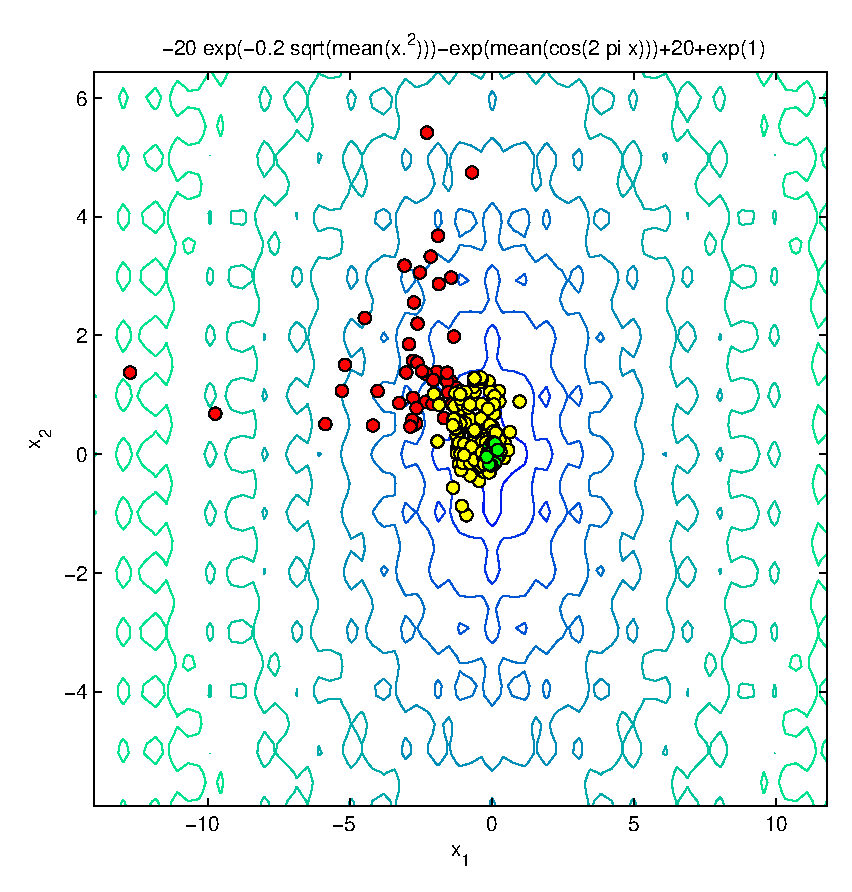
\includegraphics[scale=0.55]{ES_ackley_curvNivel.eps}
\caption{Função Ackley minimizada com Estratégias Evolutivas - Curva de Nível e indivíduos das populações}
\label{fig:ES_ackley_curvNivel}
\end{figure}

\begin{figure}
\centering
\includegraphics[scale=0.45]{ES_ackley_f.eps}
\caption{Evolução da Função Ackley avaliada para o melhor indivíduo da população em cada geração}
\label{fig:ES_ackley_f}
\end{figure}

\subsection{Simulated Annealing}


\begin{thebibliography}{1}

\bibitem{IEEEhowto:kopka}
H.~Kopka and P.~W. Daly, \emph{A Guide to \LaTeX}, 3rd~ed.\hskip 1em plus
  0.5em minus 0.4em\relax Harlow, England: Addison-Wesley, 1999.

\end{thebibliography}





\end{document}

